\phantomsection
\numberedsection{RF8 Gestión de Exportación}

\subsection*{Descripción}
El sistema permite a los usuarios exportar productos seleccionados desde Mini PIM a Amazon, configurando atributos obligatorios y opcionales de forma personalizable.

\vspace{0.15cm}

\textbf{Pre-condición}\par
El usuario ha iniciado sesión en su cuenta en Mini PIM y existen productos en el sistema con los atributos obligatorios necesarios.

\vspace{0.15cm}

\textbf{Post-condición}
\begin{itemize}
    \item Caso de éxito: Los productos seleccionados son exportados exitosamente al formato CSV requerido por Amazon y están listos para su carga.
    \item Caso mínimo: El sistema notifica al usuario cualquier error o dato faltante, permitiendo realizar las correcciones necesarias.
\end{itemize}

\textbf{Prioridad:}
Alta

\vspace{0.15cm}

\textbf{Autores:}
Diego Sicre.

\vspace{0.15cm}

\textbf{Control de cambios: } Versión 1: Definición del caso de uso.

\numberedsubsection{Escenario principal}
\begin{enumerate}
    \item El usuario accede a la sección \enquote{Productos}.
    \item El sistema muestra un listado de productos con los siguientes atributos:
    \begin{itemize}
        \item Thumbnail
        \item SKU
        \item Nombre
        \item Hasta cinco atributos de usuario.
    \end{itemize}
    \item El usuario filtra los productos\footnote{No necesariamente se tienen que seleccionar ambas opciones de filtrado para encontrar un producto. Aquí exponemos las dos alternativas combinables que tiene el usuario para filtrar.}:
    \begin{itemize}
        \item Por categoría, seleccionándola del desplegable junto al calendario.
        \item Y/O por fecha, seleccionando un día en el calendario para mostrar productos modificados desde esa fecha hasta la actualidad.
    \end{itemize}
    \item El usuario selecciona uno o más productos para exportar.
    \item El usuario hace click en el botón \enquote{CSV}.
    \item El sistema muestra un formulario para configurar el mapeo de atributos obligatorios, incluyendo:
    \begin{itemize}
        \item SKU: Se utiliza el SKU del producto en el sistema.
        \item Título: Se selecciona el \textit{Label} del producto.
        \item Fulfilled by: Nombre de la cuenta.
        \item Amazon\_SKU: Permite elegir entre SKU/GTIN.
        \item Precio: Selección de un atributo de usuario como precio del producto.
        \item Offer Price: Configuración general como \texttt{TRUE/FALSE/RANDOM}.
    \end{itemize}
    \item Si no existe ningún atributo de usuario de tipo float o entero, el sistema notifica al usuario que no se puede proceder con la exportación.
    \item El usuario confirma la configuración de mapeo obligatorio y selecciona \enquote{Continue}.
    \item El sistema permite seleccionar atributos adicionales de usuario\footnote{Se tomaron en cuenta las consideraciones descritas en \href{https://buywithprime.amazon.com/knowledge-center/csv-import?utm_medium=website\&utm_source=direct\#standalone-product}{CSV Import} de Amazon para manejar la elección de atributos adicionales de usuario correctamente.} para exportar.
    \item El usuario selecciona atributos adicionales mediante \textit{checkboxes} (opcional).
    \item El usuario selecciona \enquote{Confirmar} para finalizar la exportación.
    \item El sistema genera un archivo CSV listo para carga en Amazon.
    \item El usuario descarga el archivo generado.
\end{enumerate}

\numberedsubsection{Escenarios alternativos}
\begin{description}
    \item[4.a] No hay productos seleccionados.
    \begin{enumerate}
        \item[4.a.1] El sistema notifica al usuario que debe seleccionar al menos un producto para exportar.
    \end{enumerate}
    \item[5.a] Falta algún atributo obligatorio.
    \begin{enumerate}
        \item[5.a.1] El sistema notifica al usuario de que faltan atributos obligatorios.
    \end{enumerate}
    \item[6.a] No existe ningún atributo de usuario de tipo float o entero.
    \begin{enumerate}
        \item[6.a.1] El sistema muestra un mensaje de error indicando que no se puede proceder con la exportación, ya que no es posible mapear un precio.
    \end{enumerate}
    \item[7.a] No se seleccionan atributos adicionales.
    \begin{enumerate}
        \item[7.a.1] El sistema genera el CSV solo con los atributos obligatorios configurados.
    \end{enumerate}
    \item[8.a] El usuario no encuentra el producto al filtrar por categoría.
    \begin{enumerate}
        \item[8.a.1] El sistema muestra un mensaje indicando que no existen productos con esa categoría.
    \end{enumerate}
    \item[8.b] El usuario no encuentra el producto al filtrar por fecha.
    \begin{enumerate}
        \item[8.b.1] El sistema muestra un mensaje indicando que no hay productos disponibles en el rango seleccionado.
    \end{enumerate}
\end{description}

\numberedsubsection{Casos de Prueba}

\underline{Escenario: Principal}\par
\textbf{Dado:} Que el usuario ha iniciado sesión en Mini PIM, hay productos en el sistema, y el usuario selecciona filtros de categoría y/o fecha correctamente.  
\textbf{Entonces:} El sistema genera un CSV válido y descargable.\par

\underline{Escenario: Alternativo 6.a (Falta un atributo de tipo float o entero)}\par
\textbf{Dado:} Que el usuario intenta exportar productos.  
\textbf{Cuando:} No existe ningún atributo de usuario de tipo float o entero en el sistema.  
\textbf{Entonces:} El sistema muestra un mensaje indicando que no es posible mapear un precio y no se puede proceder con la exportación.\par

\numberedsubsection{Bocetos}
\begin{figure}[H]
    \includegraphics[width=1\linewidth]{assets/mockups/RF8 filtrado y selección de productos.png}
    \caption{Pantalla principal de exportación y formulario de configuración de mapeo}
\end{figure}


\begin{figure}[H]
    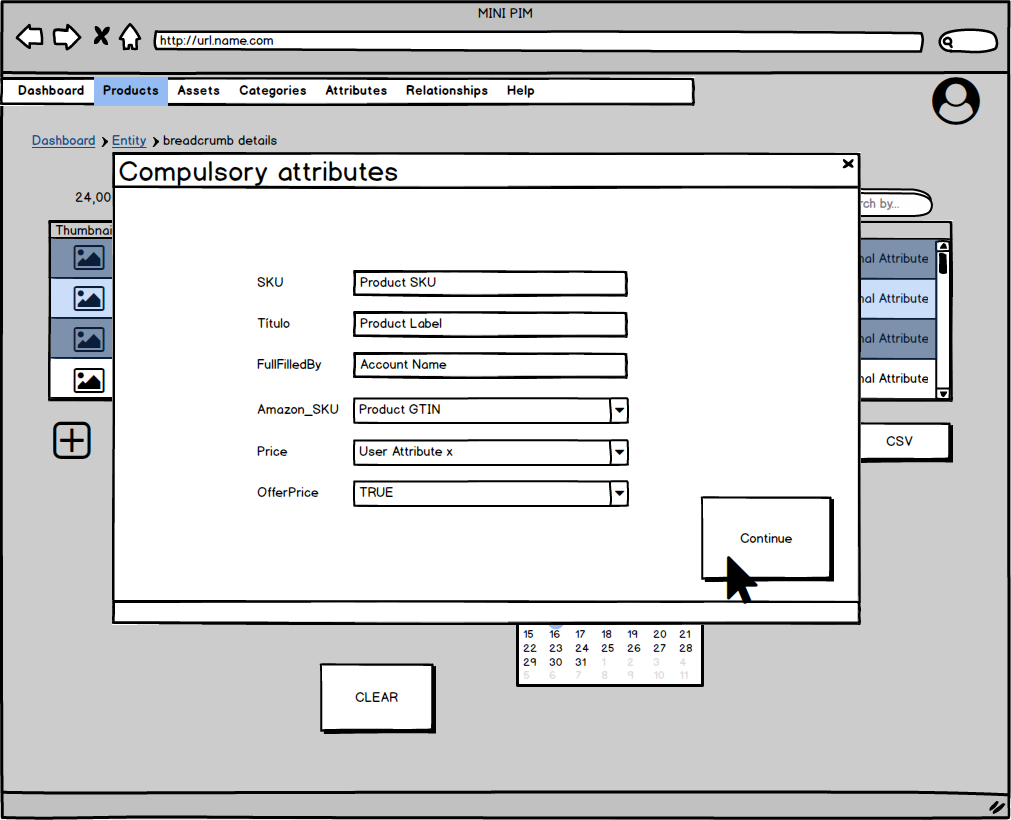
\includegraphics[width=1\linewidth]{assets/mockups/RF8 Seleccion de atributos obligatorios.png}
    \caption{Selección de atributos obligatorios en la exportación}
\end{figure}

\begin{figure}[H]
    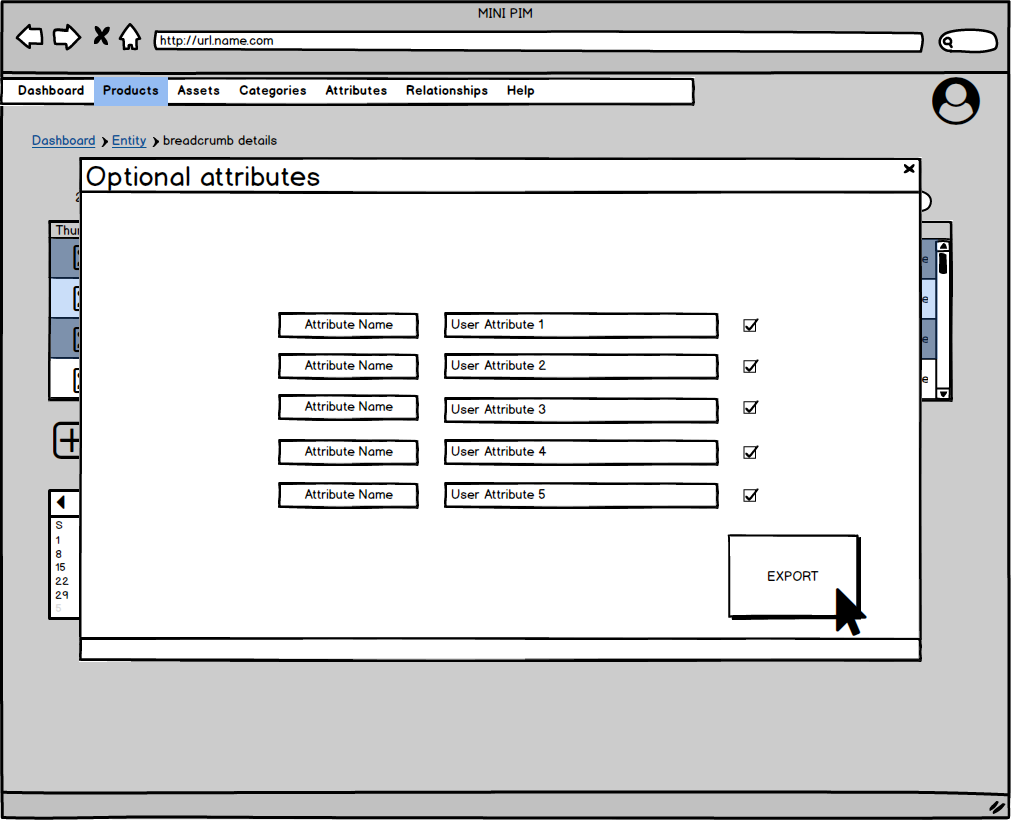
\includegraphics[width=1\linewidth]{assets/mockups/RF8 Seleccion atributos opcionales.png}
    \caption{Selección de atributos opcionales en la exportación}
\end{figure}

\numberedsubsection{Diagrama de Secuencia (por hacer)}
\begin{figure}[H]
    
\includegraphics[width=1\linewidth]{assets/umaLogo.png}
    \caption{Escenario principal para la gestión de exportación}
\end{figure}
